%!TEX root=paper.tex
\section{Introduction}

Key component of modern big data solutions are sophisticated analysis algorithms. 
Unfortunately, the search for useful patterns and peculiarities in large data sets resembles the search for a needle in a haystack. 
This challenge requires tools that are able to analyze vast amounts of data quickly. 
Many of these tools are based on statistics to extract interesting features. 

It is beneficial to apply these statistical means to the complete data set instead of smaller chunks. 
Even if the chunks cover the complete data set, important correlations between data points might get lost if chunks are treated individually. 
Moreover, the statistical tools improve their descriptive and predictive results by getting fed more data. 
The more data is available, the more likely it is that noise cancels out and that significant patterns manifest. 
However, these benefits come at the price of an increased computing time, which requires fast computer systems to make computations feasible. 

Analysis tools traditionally do not scale well for vast data sets.
Because of the exponential data growth, analytic capacities have to improve at a similar speed.
This problem can be tackled by vertical and horizontal scaling of computers.
To scale vertically means that we add more resources to a single computer.
For example, the main memory size or the CPU frequency of a computer can be increased to improve computational power.
In contrast to that, horizontal scaling refers to adding more computer nodes to a system.
By having more than one node, computational work can be split up and distributed across multiple computers.

The emerging field of multi-core and distributed systems poses new challenges for programmers.
Since they have to be able to reason about interwoven parallel control flows, parallel program development is highly cumbersome and error-prone.
Therefore, new programming models are conceived, a development that relieves the programmer from tedious low-level tasks related to parallelization such as load-balancing, scheduling, and fault tolerance.
With these new models, programmers can concentrate on the actual algorithm and use case rather than reasoning about distributed systems. 
These are the reasons why Google's MapReduce~\cite{dean:c2008a} framework and its open source re-implementation Hadoop~\cite{hadoop:2008a} became so popular among scientists as well as engineers.

MapReduce and other frameworks, however, force users to express programs in a certain way which is often not natural or intuitive to users from different domains.
Especially, in the field of data analytics and machine learning programs are usually expressed in a mathematical form.
Therefore, systems such as MATLAB~\cite{matlab} and R~\cite{r:1993a} are widely used and recognized for their fast prototyping capabilities and their extensive mathematical libraries.
However, these linear algebra systems lack proper support for automatic parallelization on large clusters and are thus restricting the user to a single workstation.
Therefore, the amount of processable data is limited to the size of a single machine's memory, which constitutes a serious drawback for real-world applications.

\begin{figure}[!h]
\centering
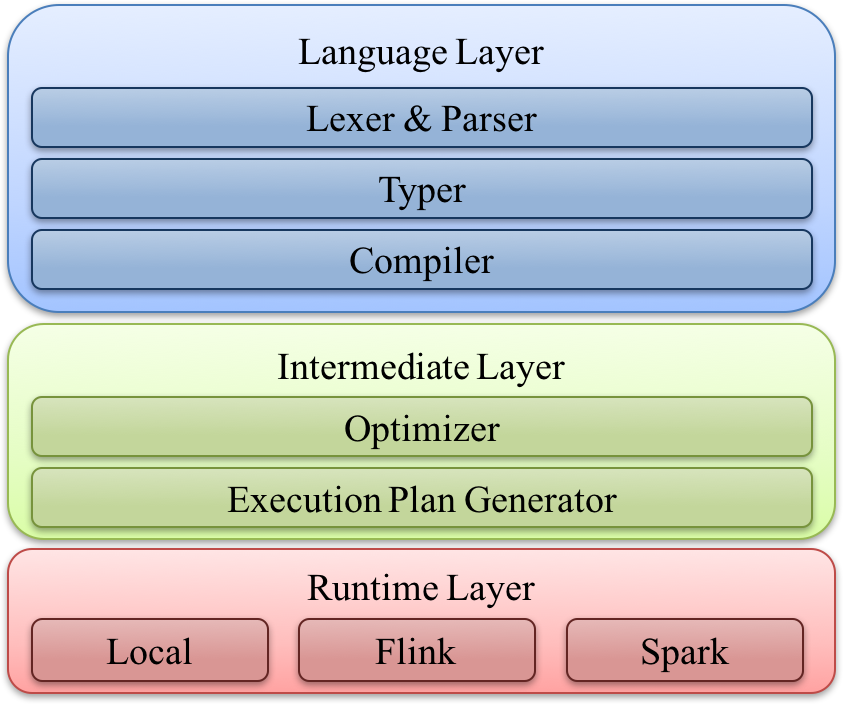
\includegraphics[height=0.15\paperheight]{images/systemArchitecture2.png}
\caption{Gilbert's system architecture consisting of the language, intermediate and runtime layer.}
\label{fig:systemArchitecture}
\end{figure}

As a solution we propose Gilbert, a distributed sparse linear algebra environment whose name is a homage to William Gilbert Strang.
Gilbert provides a MATLAB-like language for distributed sparse linear algebra operations. 
It has a layered architecture, which is shown in Figure \ref{fig:systemArchitecture}. 
The first layer is the language layer. 
This layer parses Gilbert code and compiles it into an intermediate representation (IR). 
The second layer is the intermediate layer, which is given the IR. 
The intermediate format is the ideal representation to apply language independent high-level transformations. 
The Gilbert optimizer applies several algebraic optimizations prior to the generation of the execution plan. 
The execution plan generator translates the optimized IR into an execution engine specific plan.
This execution plan is then executed on the respective back end. 

Our main contributions are:

\begin{itemize}
 \item Gilbert allows to write MATLAB-like code for sparse linear algebra and execute it on massively parallel dataflow systems.
 \item Its expressiveness allows to quickly develop scalable algorithms to analyze web-scale data.
 \item We introduce a novel fixed-point operator which replaces loops by recursion and can be efficiently parallelized.
 \item Furthermore, we demonstrate that dataflow optimizers can be used to automatically select a good matrix multiplication strategy. 
\end{itemize}

The rest of this paper is structured as follows.
In \Cref{sec:gilbertFeatures}, Gilbert's language and its features are described.
\Cref{sec:gilbertRuntime} presents how linear algebra operations are mapped to a dataflow system. Gilbert's performance and scalability is evaluated in \Cref{sec:evaluation}.
Related work is covered in \Cref{sec:relatedWork} before the work is concluded in \Cref{sec:conclusion}.